\section{Results \& Analysis}

\subsection{Main Leaderboard}

Table~\ref{tab:main} presents the full \eva{} leaderboard across 22 model configurations on the \yatcc{} workload.

\begin{table*}[t]
\centering
\small
\begin{tabular}{llrrrrrrrrrr}
\toprule
\textbf{Model} & \textbf{Backend} & \textbf{T0} & \textbf{T1} & \textbf{T2} & \textbf{T3} & \textbf{T4} & \textbf{T5} & \textbf{MR} & \textbf{PS} & \textbf{PL} & \textbf{Res} \\
\midrule
kimi-k2.6 & kimi & \textbf{100} & \textbf{100} & \textbf{100} & 98.6 & 97.4 & \textbf{100} & 99.1 & 77.8 & 99.3 & 4 \\
kimi-k2.5 & kimi & \textbf{100} & \textbf{100} & \textbf{100} & 98.6 & 95.5 & \textbf{100} & 98.5 & 77.8 & 99.0 & 4 \\
\underline{gpt-5.5} & codex & \textbf{100} & \textbf{100} & \textbf{100} & \textbf{100} & \textbf{95} & \textbf{100} & 98.5 & 100.0 & 99.2 & 0 \\
claude-sonnet-4.6 & claude & \textbf{100} & \textbf{100} & \textbf{100} & 98.6 & 94.6 & \textbf{100} & 98.3 & 77.8 & 98.9 & 4 \\
mimo-v2.5-pro & kimi & \textbf{100} & \textbf{100} & \textbf{100} & 98.6 & 94.5 & \textbf{100} & 98.2 & 77.8 & 98.9 & 4 \\
qwen3.6-flash & openhands & \textbf{100} & \textbf{100} & \textbf{100} & \textbf{100} & \textbf{92} & \textbf{100} & 97.5 & 66.7 & 98.6 & 2 \\
\underline{glm-5.1} & openhands & \textbf{100} & \textbf{100} & \textbf{100} & \textbf{100} & 91.1 & \textbf{100} & 97.3 & 100.0 & 98.5 & 0 \\
\underline{deepseek-v4-pro} & openhands & \textbf{100} & \textbf{100} & \textbf{100} & \textbf{100} & 71 & \textbf{100} & 91.4 & 66.7 & 95.2 & 0 \\
minimax-m2.7 & openhands & \textbf{100} & 61 & \textbf{100} & \textbf{93} & \textbf{98} & \textbf{100} & 90.4 & 66.7 & 91.9 & 2 \\
qwen3.6-max-preview & openhands & \textbf{100} & 61 & \textbf{100} & \textbf{97} & \textbf{94} & \textbf{100} & 90.0 & 66.7 & 92.0 & 3 \\
glm-5 & openhands & \textbf{100} & \textbf{100} & \textbf{100} & \textbf{100} & 63 & \textbf{100} & 88.8 & 66.7 & 93.8 & 1 \\
qwen3.6-plus & openhands & \textbf{100} & \textbf{100} & 74 & 73 & \textbf{81} & \textbf{100} & 85.0 & 66.7 & 88.0 & 2 \\
deepseek-v4-flash & openhands & \textbf{100} & 0 & \textbf{100} & \textbf{93} & \textbf{90} & \textbf{100} & 75.8 & 55.6 & 80.5 & 3 \\
glm-4.7 & openhands & \textbf{100} & 0 & 62 & \textbf{100} & \textbf{94} & \textbf{100} & 70.5 & 55.6 & 75.9 & 1 \\
minimax-m2.5 & openhands & \textbf{100} & \textbf{100} & 0 & 73 & \textbf{80} & \textbf{100} & 70.0 & 55.6 & 75.5 & 2 \\
qwen3.5-plus & openhands & \textbf{100} & \textbf{100} & 0 & 53 & \textbf{87} & \textbf{100} & 69.0 & 44.4 & 73.3 & 2 \\
qwen3-coder-flash & openhands & \textbf{100} & \textbf{100} & 0 & 34 & 58 & \textbf{100} & 67.5 & 33.3 & 73.7 & 3 \\
mimo-v2.5-pro & openhands & \textbf{100} & 0 & \textbf{100} & \textbf{100} & 60 & \textbf{100} & 67.0 & 44.4 & 70.8 & 3 \\
deepseek-chat & openhands & \textbf{100} & 0 & 21 & \textbf{100} & 60 & \textbf{100} & 52.2 & 44.4 & 63.5 & 2 \\
deepseek-reasoner & openhands & \textbf{100} & 0 & 21 & \textbf{100} & 60 & \textbf{100} & 52.2 & 44.4 & 63.5 & 2 \\
kimi-k2-thinking & openhands & \textbf{100} & 0 & 21 & \textbf{100} & 60 & \textbf{100} & 52.2 & 44.4 & 63.5 & 2 \\
qwen-omni-turbo & openhands & \textbf{100} & 0 & 0 & 0 & 0 & 0 & 50.9 & 33.3 & 62.6 & 2 \\
\bottomrule
\end{tabular}
\caption{\eva{} \yatcc{} leaderboard across 22 model configurations. \underline{Underlined} models achieved zero-shot pipeline success (no resurrection). \textbf{Bold} scores indicate task passing ($\geq 60\%$). MR = Mean Reward, PS = Pass Score, PL = Pipeline Score, Res = Resurrection count.}
\label{tab:main}
\end{table*}

\textbf{Key observation.}
Only 3 out of 22 configurations (GPT-5.5/Codex, deepseek-v4-pro/OpenHands, and glm-5.1/OpenHands) achieve zero-shot pipeline success without any resurrection.
The top 5 positions are dominated by Kimi CLI backend configurations (kimi-k2.6, kimi-k2.5, mimo-v2.5-pro), demonstrating that scaffold choice significantly impacts outcomes---the same model \texttt{mimo-v2.5-pro} scores 98.2 on Kimi CLI versus 67.0 on OpenHands, a 31.2-point gap.

\subsection{Resurrection Recovers Hidden Downstream Capability}

Figure~\ref{fig:resurrection_gain} shows the per-task score improvement when resurrection is enabled versus the no-resurrection setting.
Without resurrection, 19 out of 22 configurations cannot reach the full pipeline depth of 6 tasks; the median zero-shot pipeline depth is only 1 task.
With resurrection, all configurations can be evaluated at every downstream node, recovering diagnostic signal that would otherwise be lost.

\begin{figure}[t]
\centering
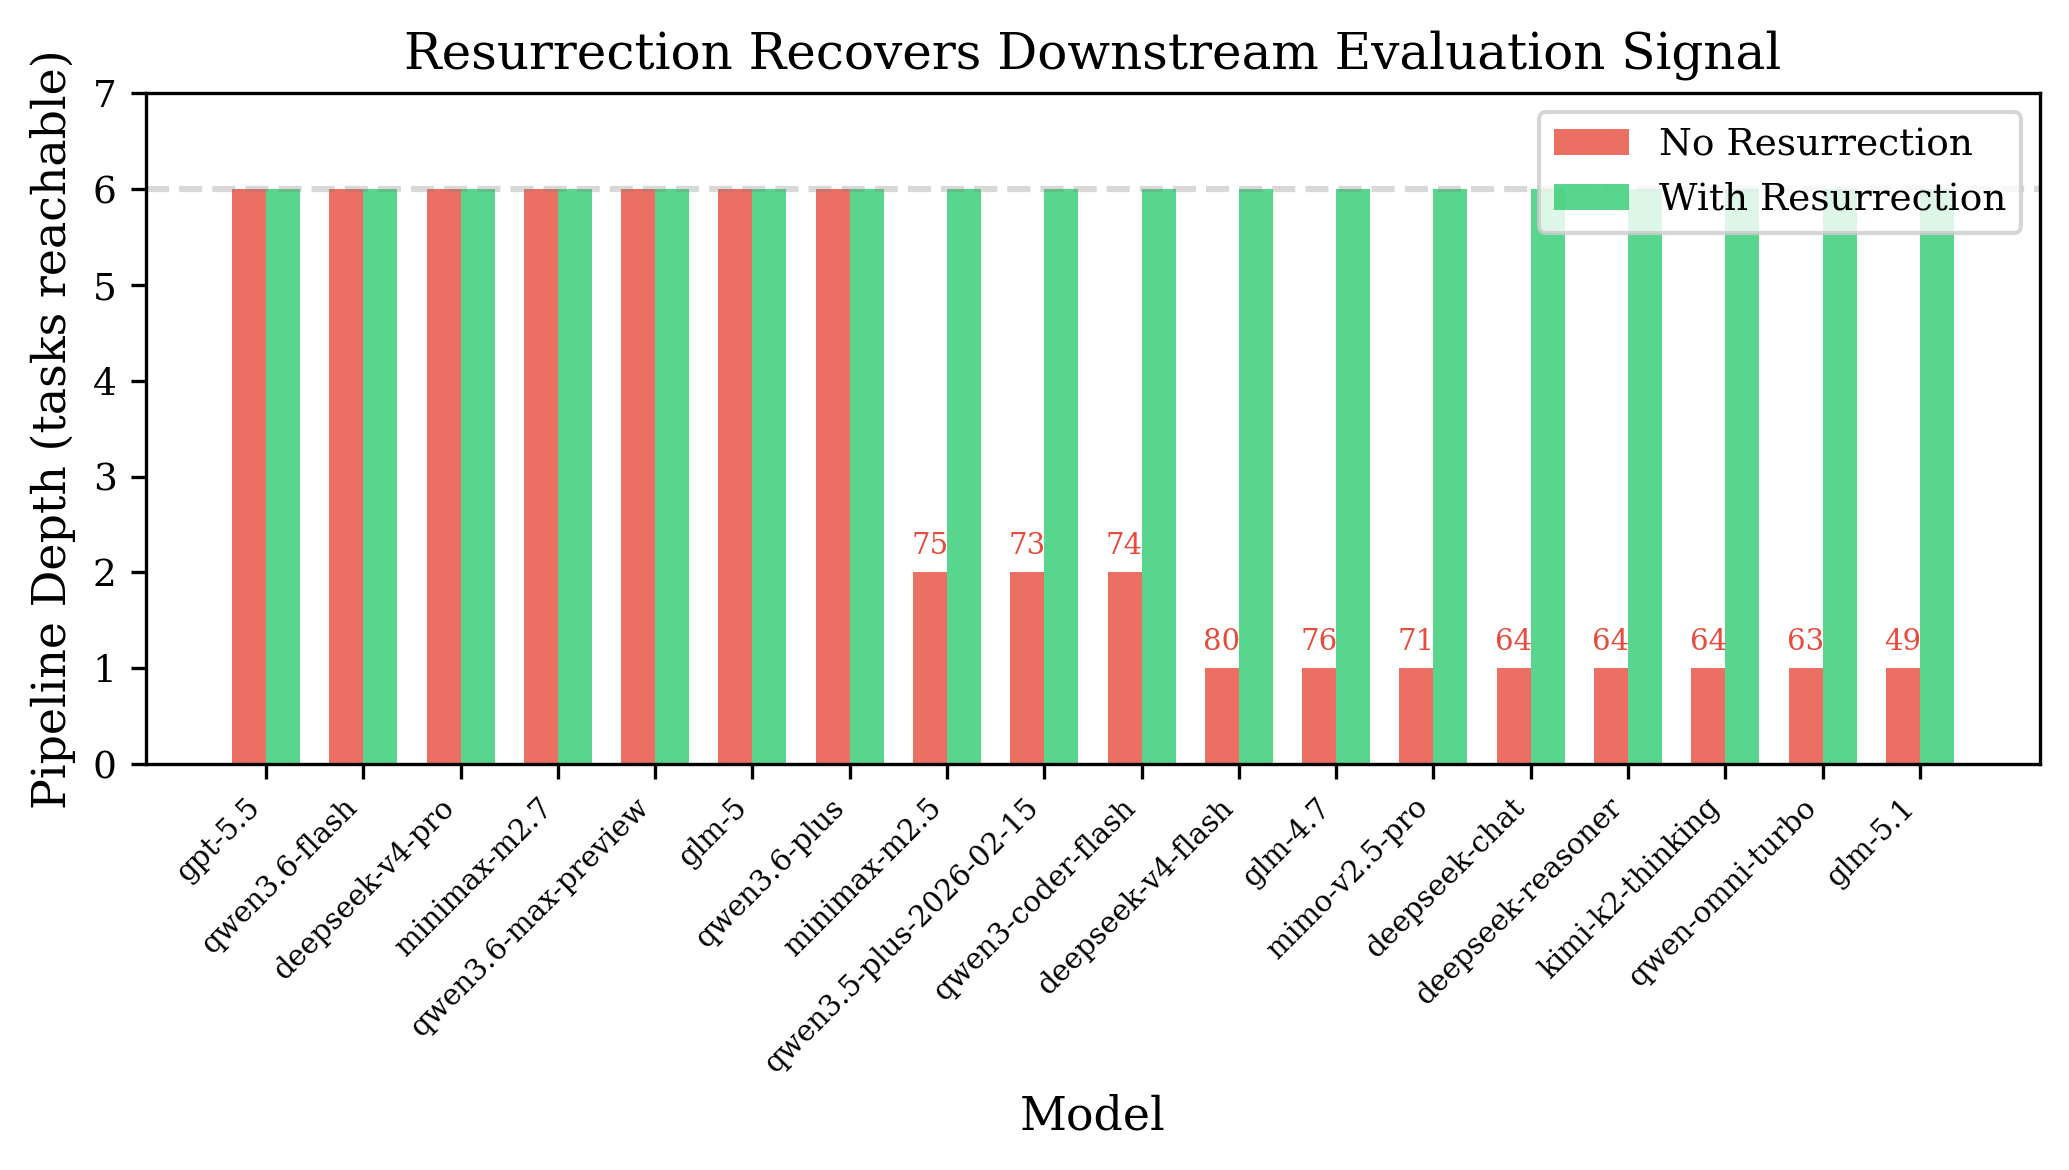
\includegraphics[width=\linewidth]{figures/fig_resurrection_gain.png}
\caption{Resurrection recovers downstream evaluation signal. Without resurrection, most agents can only be evaluated at 1--2 tasks before cascading failure blocks further measurement. With resurrection, all 6 tasks become reachable, revealing hidden downstream capability.}
\label{fig:resurrection_gain}
\end{figure}

The most striking example is \texttt{claude-sonnet-4.6}: without resurrection, it scores 0 on Tasks~3--5 (pipeline depth = 3, PL = 50.0), but after resurrection at Tasks~2--5, achieves 98.6 on Task~3, 94.6 on Task~4, and 100 on Task~5 (PL = 98.9, MR = 98.3, Rank~4).
This represents a \emph{48.9-point} pipeline score improvement---demonstrating that the agent's failure at Task~2 was purely a predecessor effect, not downstream incapability.

\textbf{Systematic analysis.}
The resurrection gain is not limited to cherry-picked examples: 17 out of 19 non-zero-shot configurations achieve $>40$-point pipeline score improvement with resurrection, and the median gain is 73.65 points.
Only the three zero-shot configurations show zero gain.
The mean resurrection gain across all configurations is 71.55 points, demonstrating that cascading failure systematically obscures downstream capability in serial workloads---resurrection recovers this lost signal at scale.

\subsection{Serial Evaluation Preserves Overall Ranking but Reveals Specific Failure Patterns}

To test whether serial evaluation provides different information than static evaluation, we define an \emph{independent-task baseline}: for each model, we compute the average of per-task scores obtained \emph{with resurrection} (i.e., with golden prerequisites provided at each task), which measures each task's capability in isolation.
A Kendall $\tau$ correlation of 0.763 ($p < 0.001$) between the no-resurrection serial ranking and the independent-task ranking confirms that the two rankings are \emph{strongly correlated}---serial evaluation does not wholesale reorder the leaderboard.
However, $\tau = 0.763$ is not 1.0: specific models experience large directional shifts invisible in aggregate correlation statistics.

\begin{figure}[t]
\centering
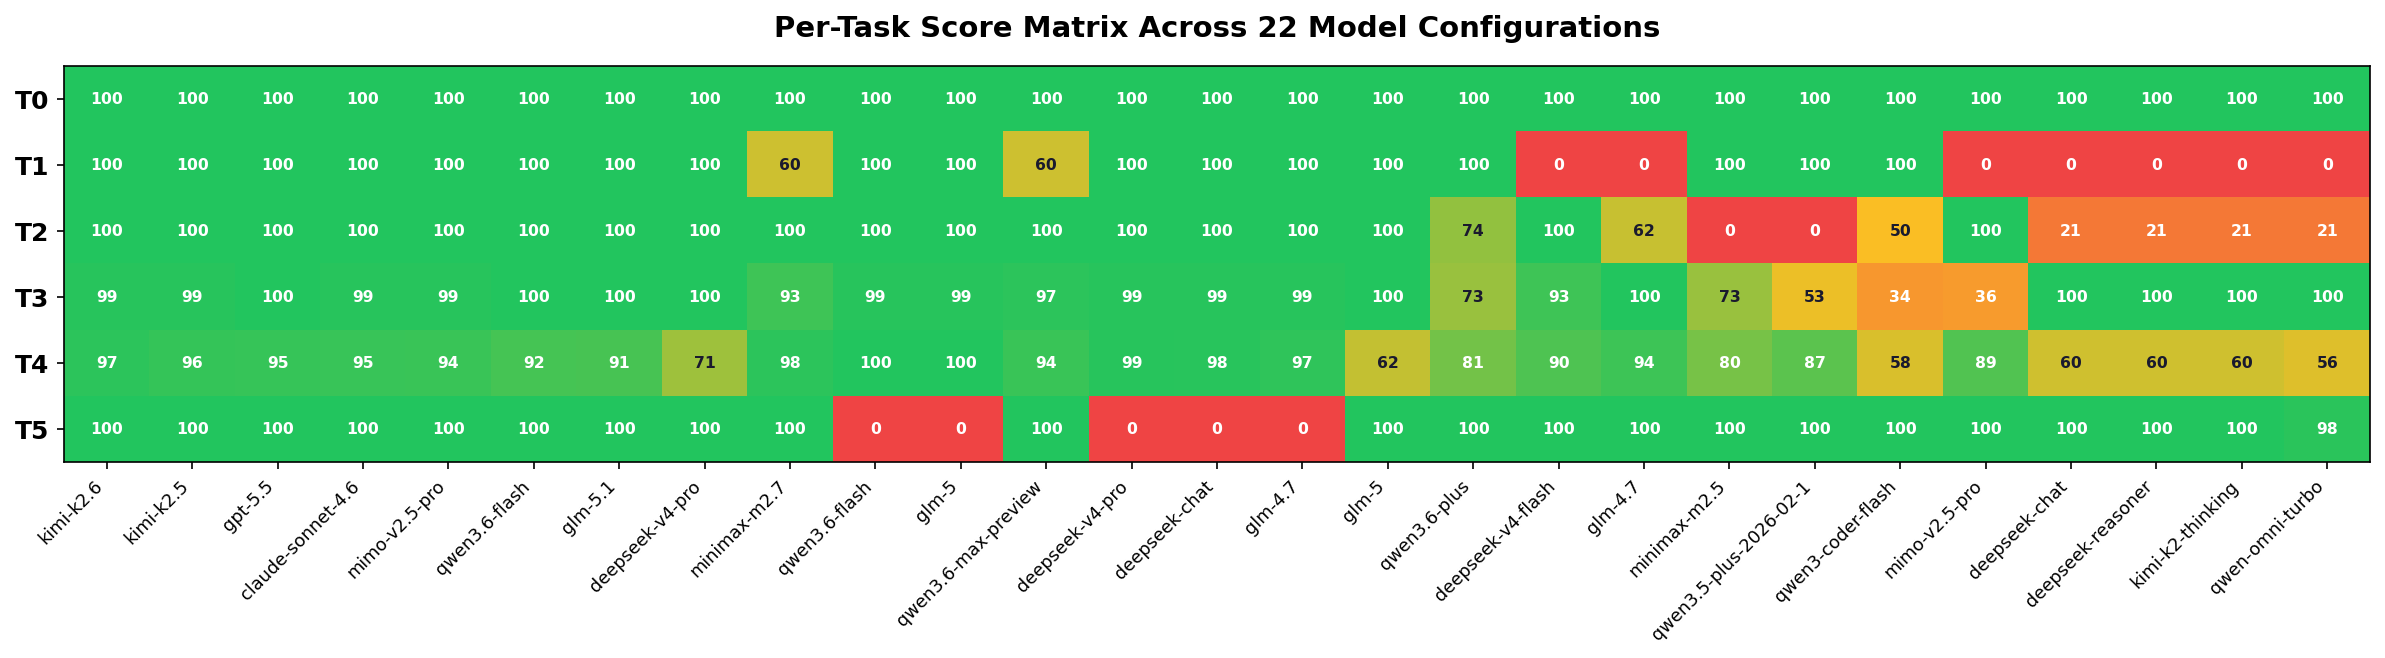
\includegraphics[width=\linewidth]{figures/fig_score_heatmap.png}
\caption{Per-task score matrix across 22 configurations. The heatmap reveals distinct failure patterns: some models fail at early tasks (T1/T2) while others fail at later tasks (T4), demonstrating that serial evaluation captures qualitatively different information than independent-task benchmarks.}
\label{fig:ranking_shift}
\end{figure}

The most dramatic rank shifts occur for models that fail at early tasks but demonstrate strong downstream capability:
\texttt{deepseek-v4-flash} drops from independent-task rank~8 to no-resurrection rank~14 (shift of 6 positions), because its Task~1 failure blocks the entire pipeline despite achieving 93.2\% on Task~3 and 89.5\% on Task~4 with resurrection.
A Wilcoxon signed-rank test on the paired rank differences yields $W = 34.5$, $p = 0.44$, indicating that the \emph{overall} ranking structure is preserved, but individual models can experience large directional shifts.
The key finding is that serial evaluation \emph{selectively penalizes} models with early-stage failures while \emph{rewarding} those with consistent cross-task continuity.

\subsection{Model--Scaffold Interaction}

The choice of agent scaffold significantly affects outcomes.
The same model (\texttt{mimo-v2.5-pro}) scores 67.0 on OpenHands versus 98.2 on Kimi CLI---a 31.2-point gap attributable entirely to scaffold design differences in action space, retry logic, and context management.
The top 5 positions are occupied by CLI-based backends (Kimi CLI: 3, Codex: 1, Claude Code: 1), while OpenHands-based configurations occupy ranks 6 and below.
This confirms that \emph{scaffold design is an independent variable} that must be controlled and reported in evaluation frameworks.

\subsection{\yatcc{} vs. \yatcc{}-Hard: The Scaffolding Gap}

Table~\ref{tab:hard} presents the \yatcc{}-Hard leaderboard across 18 model configurations.
The difficulty gap between the two workloads quantifies the value of scaffolding in agentic coding tasks.

\begin{table}[t]
\centering
\small
\begin{tabular}{lrrrrrrrr}
\toprule
\textbf{Model} & \textbf{T0} & \textbf{T1} & \textbf{T2} & \textbf{T3} & \textbf{T4} & \textbf{T5} & \textbf{PL} & \textbf{Res} \\
\midrule
qwen3.6-max-preview & 100 & 100 & 86.0 & 86.3 & 94.5 & 100 & 94.5 & 0 \\
deepseek-v4-pro & 100 & 100 & 79.5 & 87.7 & 66.5 & 98.4 & 88.7 & 1 \\
glm-5.1 & 100 & 100 & 89.1 & 91.8 & 42.8 & 100 & 87.3 & 2 \\
deepseek-v4-flash & 100 & 100 & 77.8 & 89.0 & 61.1 & 60.9 & 81.5 & 0 \\
qwen3.6-plus & 100 & 100 & 77.1 & 19.2 & 67.3 & 96.9 & 76.7 & 2 \\
glm-5 & 100 & 100 & 65.7 & 65.8 & 66.4 & 50.0 & 74.6 & 2 \\
minimax-m2.7 & 100 & 80.4 & 33.5 & 41.1 & 66.1 & 60.9 & 63.7 & 2 \\
kimi-k2.6 & 100 & 100 & 18.0 & 41.1 & 55.2 & 75.0 & 64.9 & 3 \\
\bottomrule
\end{tabular}
\caption{\yatcc{}-Hard leaderboard (top 8 of 18). Scores drop significantly compared to \yatcc{}---the best model achieves only PL=94.5 on Hard vs.\ PL=99.3 on \yatcc{}.}
\label{tab:hard}
\end{table}

\textbf{Key observation.}
The best \yatcc{}-Hard score (PL=94.5 by \texttt{qwen3.6-max-preview}) is 4.8 points below the best \yatcc{} score (PL=99.3 by \texttt{kimi-k2.6}).
More dramatically, models that excel on \yatcc{} often collapse on \yatcc{}-Hard: \texttt{kimi-k2.6} drops from PL=99.3 (Rank~1 on \yatcc{}) to PL=64.9 (Rank~8 on \yatcc{}-Hard), a 34.4-point decline.
Similarly, \texttt{mimo-v2.5-pro} drops from PL=98.9 (Rank~5 on \yatcc{}) to PL=0.0 on \yatcc{}-Hard---a complete collapse.
This gap reveals that scaffolded starter code provides substantial leverage, and that models appearing capable when filling in blanks may lack the architectural reasoning required for full from-scratch implementation.

The resurrection mechanism is equally critical on \yatcc{}-Hard: 12 out of 18 configurations require at least one resurrection.
This confirms that cascading failure is a workload-independent phenomenon---it affects both scaffolded and from-scratch settings, and resurrection provides diagnostic value in both contexts.
Notably, 6 out of 18 models score 0.0 on \yatcc{}-Hard (including \texttt{mimo-v2.5-pro}, \texttt{kimi-k2-thinking}, and \texttt{deepseek-chat}), indicating a fundamental capability threshold that current models cannot cross without scaffolding.
% GOAL: Token/turn/retry analysis, failure taxonomy, cost-performance frontier.
% COMPRESSED to fit within 9-page body limit.

\subsection{Cost-Performance Frontier}

Figure~\ref{fig:cost_frontier} plots total elapsed time against pipeline score for all evaluated configurations.
Two patterns emerge:
(1)~\emph{high-score configurations are not always low-cost}---deepseek-reasoner achieves PL=63.5 but requires 15,987 seconds and 252 build attempts, while qwen3.6-flash achieves PL=98.6 in only 1,421 seconds with 52 builds;
(2)~\emph{cost efficiency varies dramatically}---the same pipeline score of 63.5 is achieved by three models with elapsed times ranging from 1,909s to 15,987s (an 8x difference).

\textbf{Process cost does not predict outcome.}
A linear regression of build count against pipeline score yields $R^2 = 0.003$ ($p = 0.82$); elapsed time against pipeline score yields $R^2 < 0.001$ ($p = 0.98$).
The combined model explains only 0.7\% of score variance.
This \emph{decoupling} is itself a diagnostic finding: agents that invest more computational budget (time, builds, retries) do not systematically achieve better outcomes.
The relationship is not monotonic---some agents achieve high scores with minimal effort (efficient solvers), while others exhaust their budget without progress (process collapse).
This demonstrates that process metrics capture \emph{qualitatively distinct} information from outcome metrics---not because they predict scores, but because they reveal \emph{how} agents arrive at their outcomes.
Two agents with identical pipeline scores may have radically different process profiles (efficient solver vs.\ persistent searcher), and this distinction is invisible to outcome-only evaluation but critical for deployment decisions (cost budgeting, timeout setting, scaffold optimization).
Process metrics thus serve a \emph{diagnostic} rather than \emph{predictive} role: they do not explain \emph{why} an agent succeeds, but they reveal \emph{how} it attempts to succeed, enabling targeted intervention when the process profile indicates inefficiency or collapse.

\begin{figure}[t]
\centering
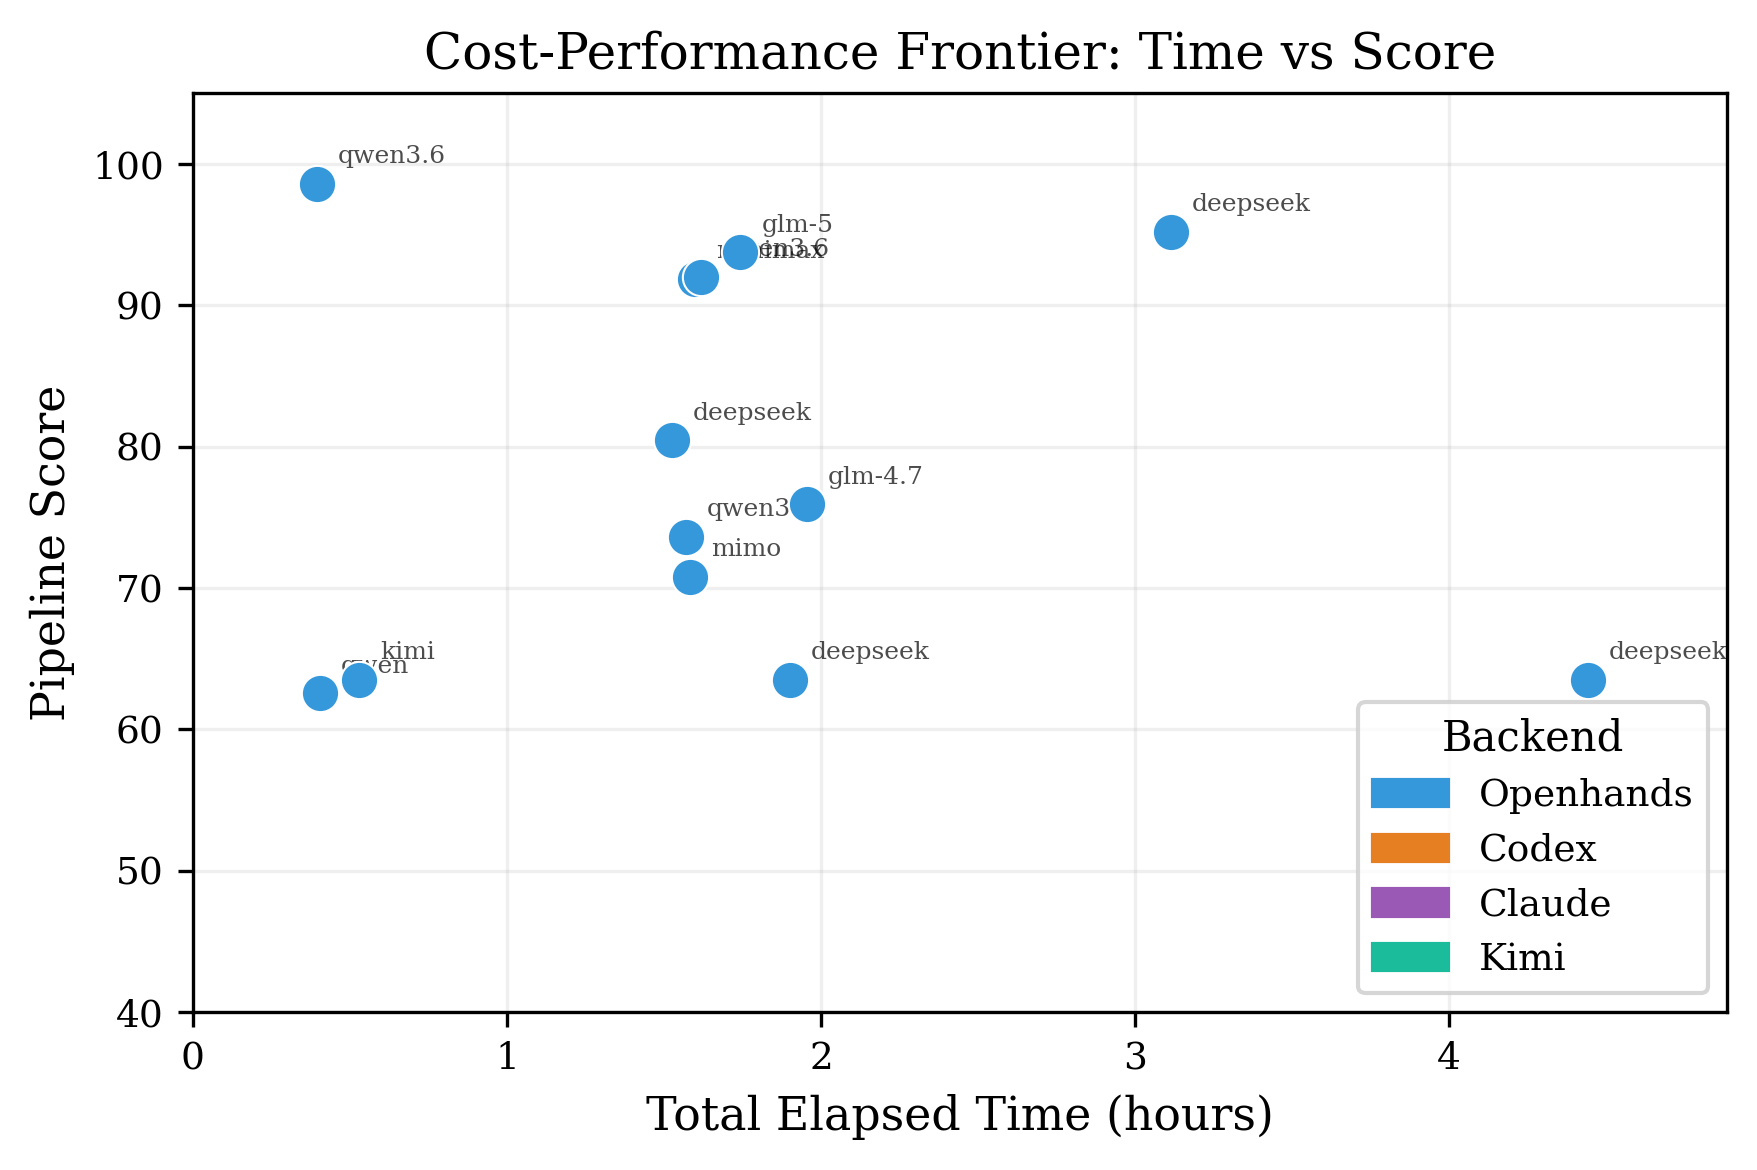
\includegraphics[width=\linewidth]{figures/fig_cost_performance.png}
\caption{Cost-performance frontier: elapsed time vs.\ pipeline score. The Pareto frontier highlights configurations achieving the best performance per unit time. The 8x cost difference between similarly-scoring agents (kimi-k2-thinking at 1,909s vs.\ deepseek-reasoner at 15,987s, both PL$\approx$63.5) demonstrates that outcome-only evaluation misses critical deployment information.}
\label{fig:cost_frontier}
\end{figure}

Build attempt counts reveal distinct agent behaviors: \emph{efficient solvers} (GPT-5.5: 80 builds, qwen3.6-flash: 52 builds) achieve high scores with minimal retries; \emph{persistent searchers} (deepseek-v4-flash: 181 builds, deepseek-reasoner: 252 builds) achieve moderate scores through exhaustive search; and \emph{collapsed agents} exhaust builds without progress. Agents that repeatedly build without modifying code exhibit \emph{process collapse}---a failure mode where the action loop decouples from productive problem-solving.

\subsection{Failure Taxonomy}

We categorize agent failures into five types: (1)~\emph{predecessor failure} (downstream unreachable), (2)~\emph{task-local reasoning failure} (cannot solve despite correct prerequisites), (3)~\emph{execution failure} (build/dependency errors), (4)~\emph{process collapse} (max-turn exhaustion, search loops), and (5)~\emph{cost overrun} (budget exhausted).

\begin{figure}[t]
\centering
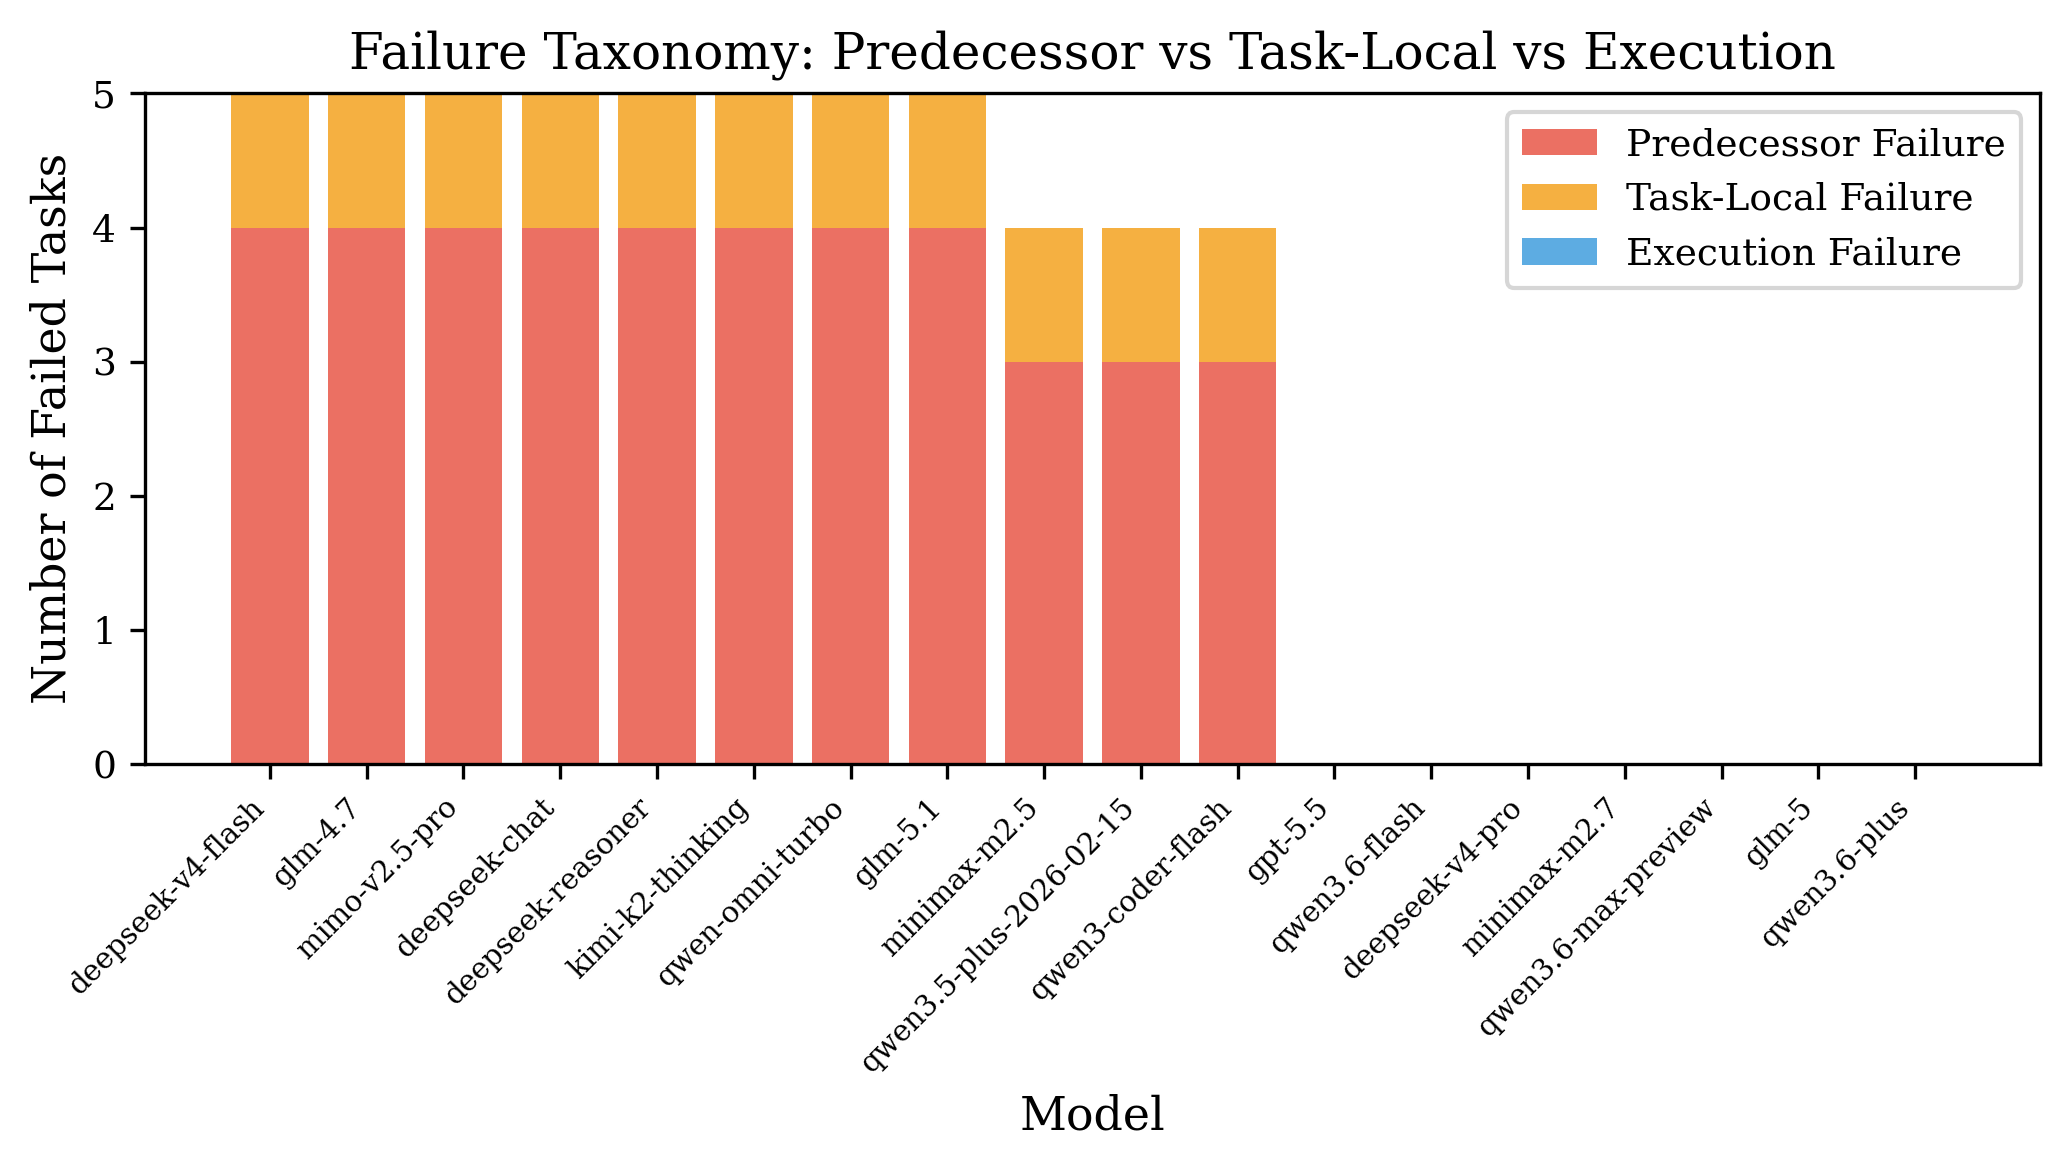
\includegraphics[width=\linewidth]{figures/fig_failure_taxonomy.png}
\caption{Failure taxonomy composition. Predecessor failure dominates without resurrection but is largely eliminated by resurrection, revealing the underlying task-local and execution failure distribution.}
\label{fig:failure_taxonomy}
\end{figure}

Figure~\ref{fig:failure_taxonomy} shows that predecessor failure dominates in the no-resurrection setting but is largely eliminated by resurrection, revealing the underlying distribution of task-local and execution failures. Process collapse is more prevalent in framework-based agents with unlimited iteration budgets, suggesting that scaffold design affects not just \emph{whether} the agent succeeds, but \emph{how} it fails.